\documentclass[11pt,a4paper,oneside]{report}
\usepackage[T1]{fontenc}
\usepackage[utf8]{inputenc}
\usepackage[french,english]{babel}
\usepackage[babel=true,kerning=true]{microtype}
\usepackage[usenames,dvipsnames,svgnames,table]{xcolor}
\usepackage[colorlinks,linkcolor={blue!30!black},citecolor={blue!50!black},urlcolor={blue!80!black}]{hyperref}
\usepackage{amsmath,amsfonts,amssymb,array,graphicx,caption,lmodern,subcaption,tikz,url,xspace,wrapfig}
\usepackage{textcomp,rotating,epic,pdfpages,listings,diagbox,multirow,float}

\usepackage[top=25mm,bottom=25mm,left=25mm,right=25mm]{geometry}

\parskip=6pt % adds vertical space between paragraphs

\DeclareMathOperator{\e}{e}

\usepackage{fancyhdr}
\headheight=14pt
\lhead{\textsc{EXAFS Practical - Report}}
\chead{}

\begin{document}

\pagenumbering{gobble}  % Pas de numérotation
\begin{titlepage}
    \vspace*{50px}
    
\includegraphics[height=80px]{Images/logo_phelma.pdf}
    \vspace*{-80px}
\begin{flushright}
%     \vspace*{60px}
    
\includegraphics[height=65px]{Images/CIME.jpg}
\end{flushright}

\vspace*{2cm}

\begin{center}
\rule{\linewidth}{0.5mm}\\[0.4cm]
{\huge{\bfseries Compte Rendu}\\[0.4cm]
\textsc{TP Simulation électronique}\\[0.4cm]}
\rule{\linewidth}{0.5mm}\\[0.5cm]

\LARGE{\textsc{Nicolas Paillet, Félix Piédallu \& Giulia Rizzo}}\\[0.7cm]
\large{\textsc{2015-2016}}\\[2cm]

\Large{~}\\[1cm]
% 
\includegraphics[width=0.4\textwidth]{Images/CIME.jpg}\\[1cm]
%
 \large{Encadrant : Marco Pala}\\[2cm]
%

\end{center}
\end{titlepage}

\tableofcontents        % Table des matières avec liens, générée automatiquement.
\newpage
\pagenumbering{arabic}  % Numérotation de retour !

\pagestyle{fancy}

\chapter*{Introduction}
\addcontentsline{toc}{chapter}{Introduction}
ESRF is the European Structure Radiation Facility. It is an international (mostly European) structure which produce high energy X-Ray used for several application in research and inductry. Thanks to the brillance and quality of X-Ray produces, researchers are able, in beamlines to reach and study the structure of matter. Several ways to characterize matter can be done with X-Rays produced by the Synchrotron, but during this practical work, we will focus on a mehod called EXAFS.

Extended X-Ray Absorption Fine Structure (EXAFS) is a spectroscopic method to caracterize elements of a sample (fluid or solid). The sample is placed on the trajectory of a X-Ray beam, the insensity of the X-Ray is mesured before and after the sample, it gives us the absorption of the X-Ray while passing through the sample.\\
The sample is scanned by X-Rays of different energies. In the EXAFS domain, kinetic energy of photoelectron goes from 50 eV to 1000 eV approximately.

We will first present the principles of functioning of the synchrotron used and then the theoretical aspects of the EXAFS. Then, we will show how to prepare the line for measurements, how to make samples and some exploitations of the results given by the EXAFS method.


\chapter{Synchrotron and EXAFS method}

\section{Operating principle Grenoble Synchrotron}

ESRF is a synchrotron, so it mostly consists in a LINear ACcelerator (LINAC), a booster ring and a storage ring :
\begin{itemize}
    \item LINAC: At the beginning, an electron gun generates electron and sends them to the LINAC where they are accelerated by an electromagnetic field. At ESRF, electron gun is a 100 keV triode gun and there are two 6-meters acceleration sections of 35 MW each to give electron an energy of 200 MeV.
    \item Booster ring: when electrons have been pre-accelerated in the LINAC, they enter in the booster ring (300 meters circumference) where they will be accelerated to reach a speed close to  the speed of light at an energy of 6 GeV.
    \item Storage ring: It is the last and biggest ring (844.4 meters circumference). In this ring, electrons alternate straight lines and bending sections. The ESRF synchrotron storage ring consists in 64 bending magnets. On the straight lines, there are 320 quadrupoles to keep the beam focused, 224 sextupoles to avoid chromatic aberration and also ondulators and wigglers which both force the electrons to have a sinusoidal trajectory instead of a straight one.
\end{itemize}

When electrons turn and slow down, they emit X-Rays braking radiation. These X-Rays are guided to the beamlines, where they will go through the samples to analyse.

The Hall where all experiments lines (beamlines) are regrouped can be seen in the figure \ref{Hall}.

\begin{figure}[H]
    \begin{center}
        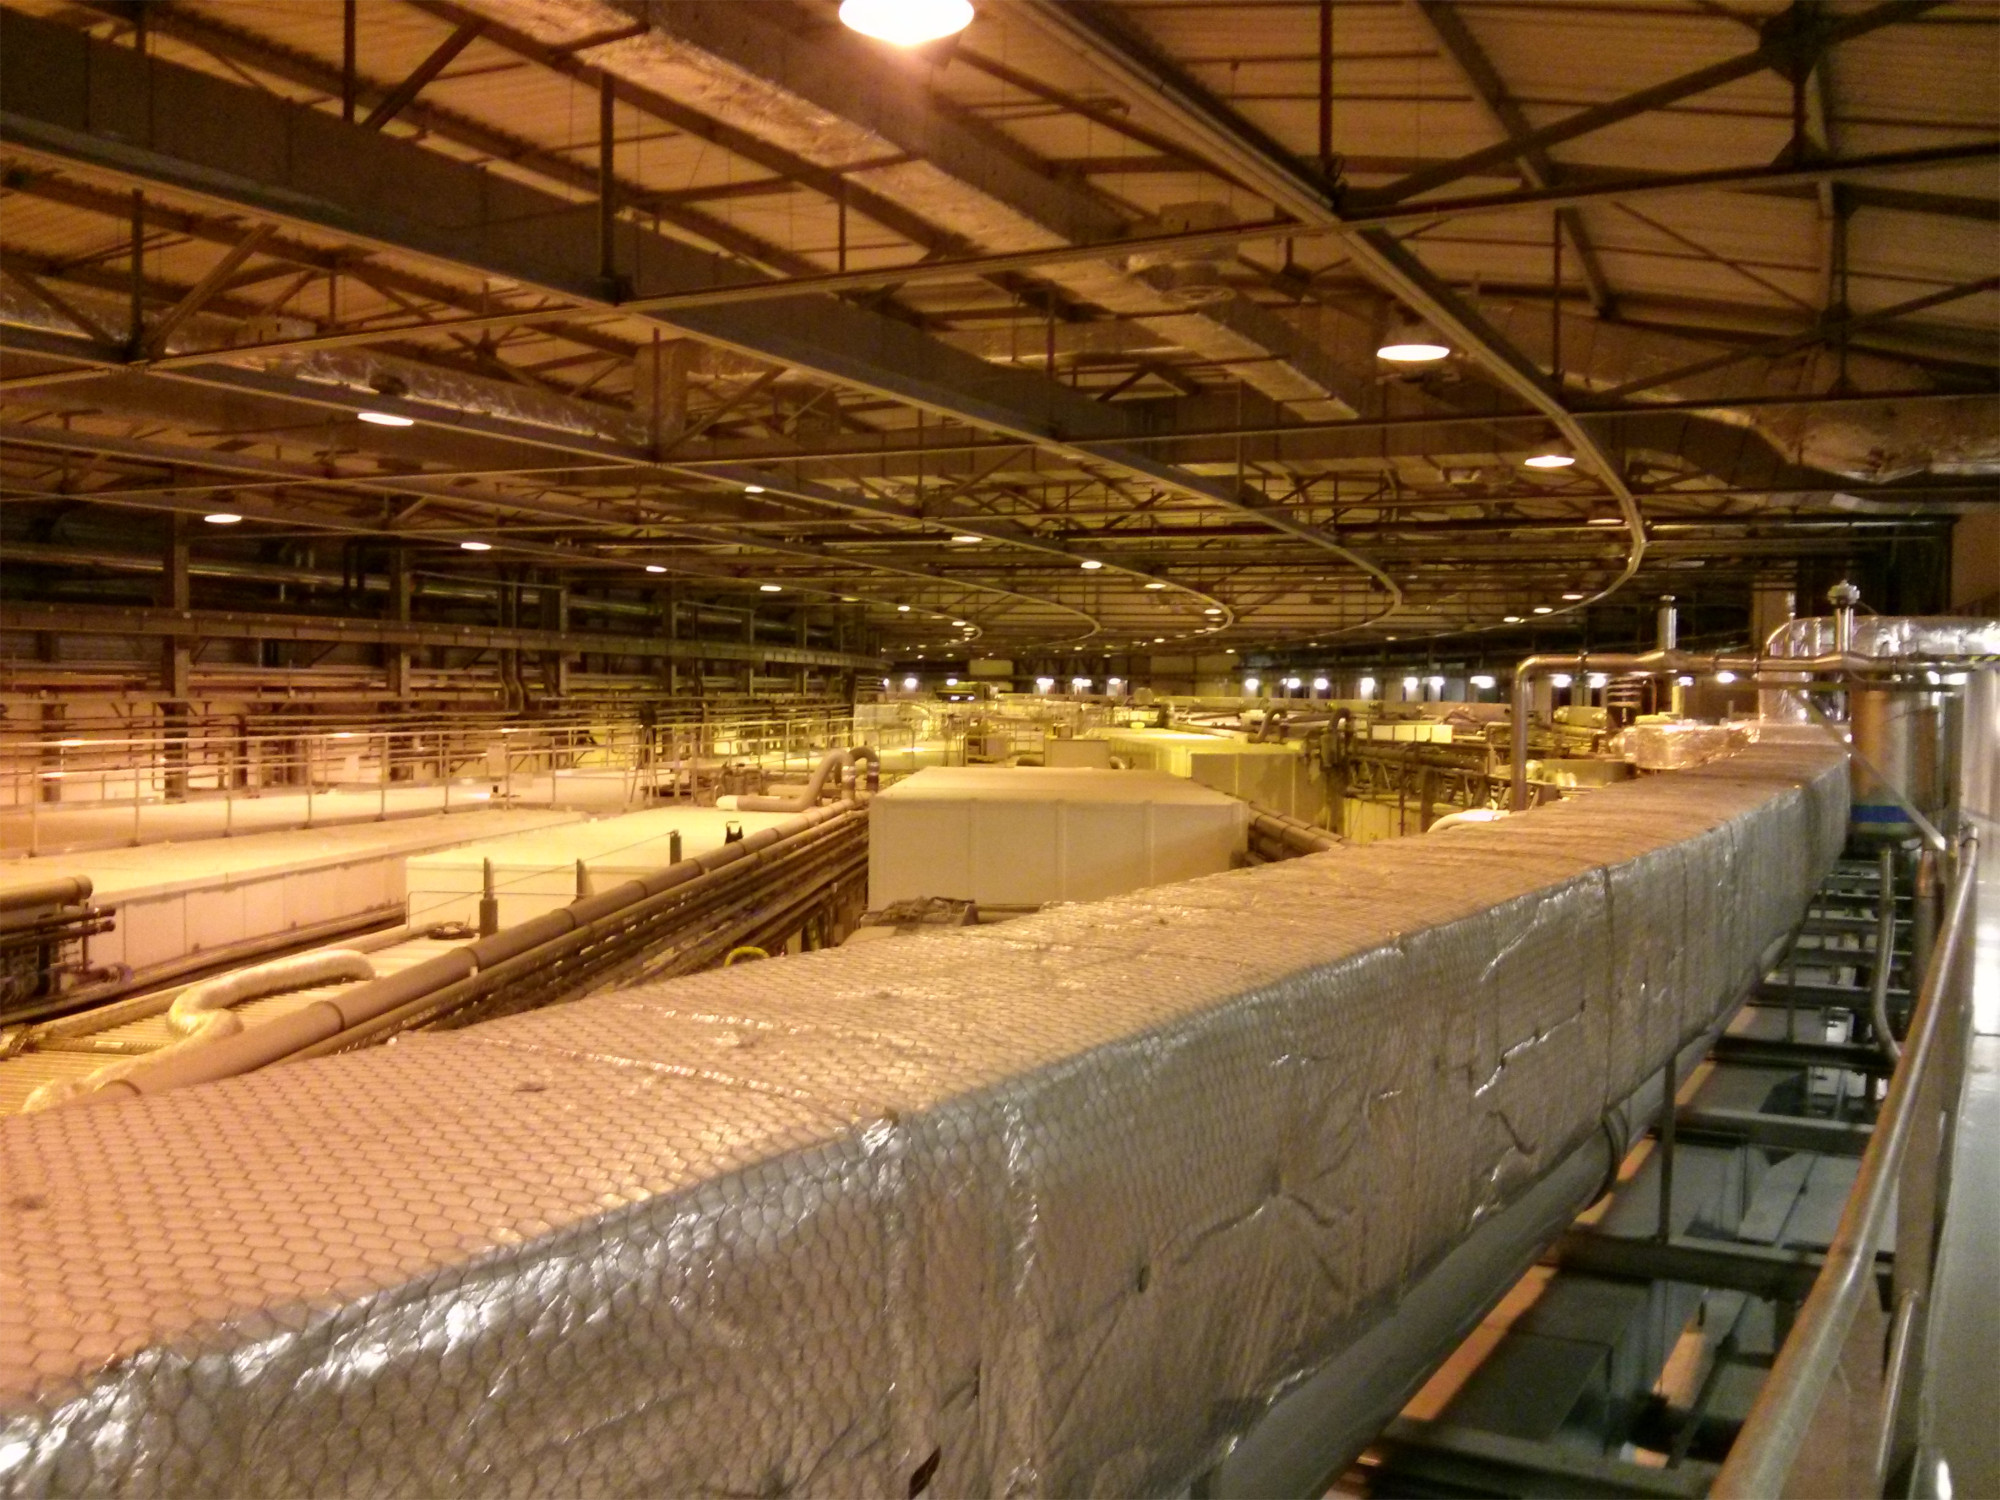
\includegraphics[width=0.8\textwidth]{Images/IMG_20151210_213319.jpg}
        \caption{Hall of experiments (ESRF Grenoble)}
        \label{Hall}
    \end{center}
\end{figure}


Figure \ref{Incident}, shows the beginning of the beamline we used (BM23). The tunnel on the right is the exit of the  storage ring which corresponds to the entrance in the beamline and which is also the first component that focuses the X-Ray beam in the beamline.

\begin{figure}[H]
    \begin{center}
        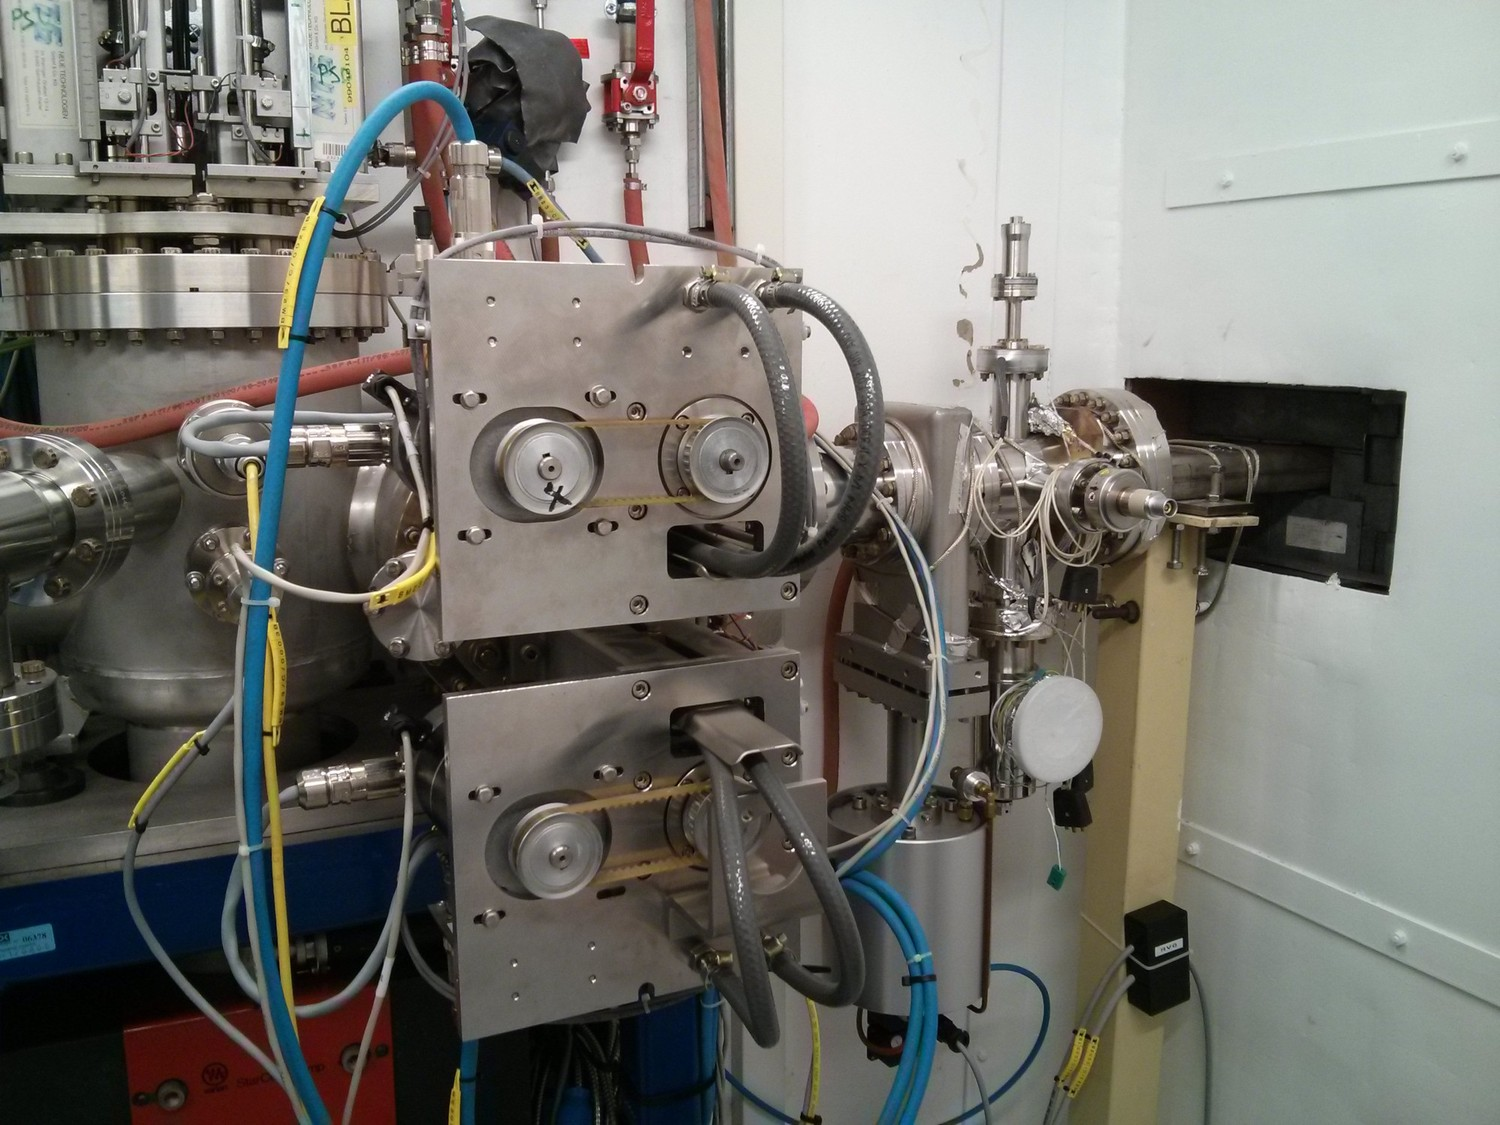
\includegraphics[scale=0.13]{Images/IMG_20151210_202655.jpg}
        \caption{Beamline enter for X-Ray radiation and focus beam straight in the beamline}
        \label{Incident}
    \end{center}
\end{figure}


Then, there is a serie of optics components that will prepare the X-Ray beam, so that is becomes usable for experiments. The first component is the monochromator (Shown in Figure \ref{monochromateur}). When the breaking radiation is created, it has a wide band of energy, the monochromator uses Bragg reflection to keep only one particular energy (wavelength) of X-Rays. Bragg's law is the equation \ref{Bragg}. This equation shows that the dispersion in wavelength $\lambda$ cause a dispersion in reflection angle. The monochromator uses this to shut down X-Rays that do not have the wanted energy.

\begin{equation}
    2d sin \theta = n \lambda  \label{Bragg}
\end{equation}
With:\\
d: distance between the two mirors\\
$\theta$: reflection angle\\
n: diffraction order\\
$\lambda$: wavelength\\


\begin{figure}[H]
    \begin{center}
        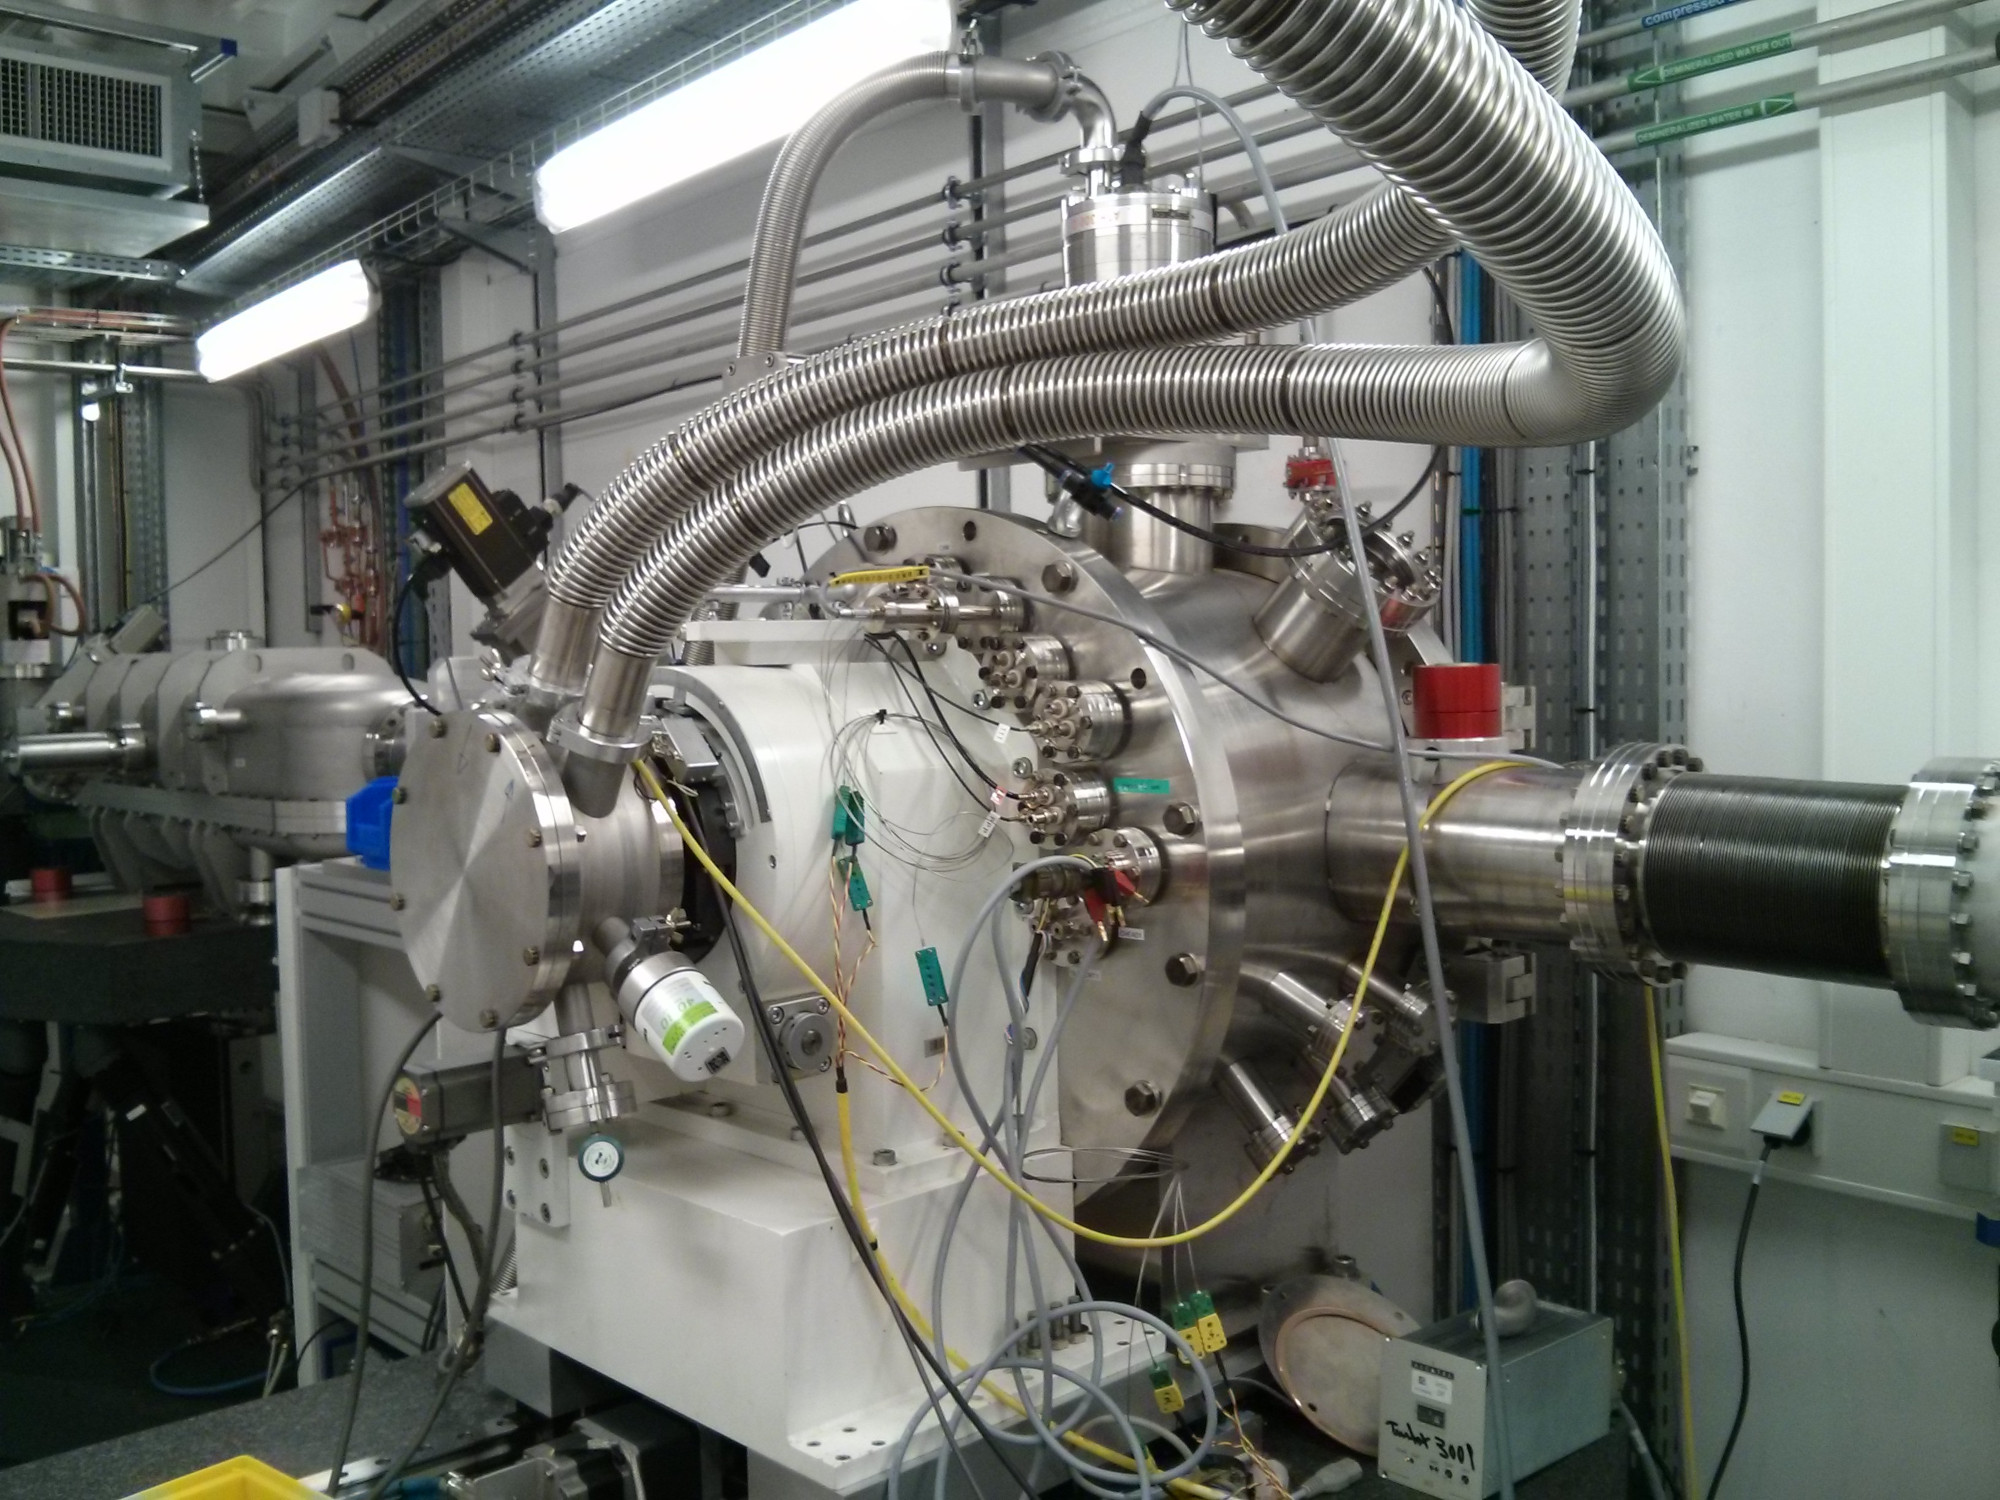
\includegraphics[scale=0.13]{Images/IMG_20151210_202721.jpg}
        \caption{Monochromator}
        \label{monochromateur}
    \end{center}
\end{figure}


Just after the monochromator, it is necessary to put a diffraction grating (figure \ref{Reseau_diffract}) to select only the first diffraction order n=1 (delete harmonics).

\begin{figure}[H]
    \begin{center}
        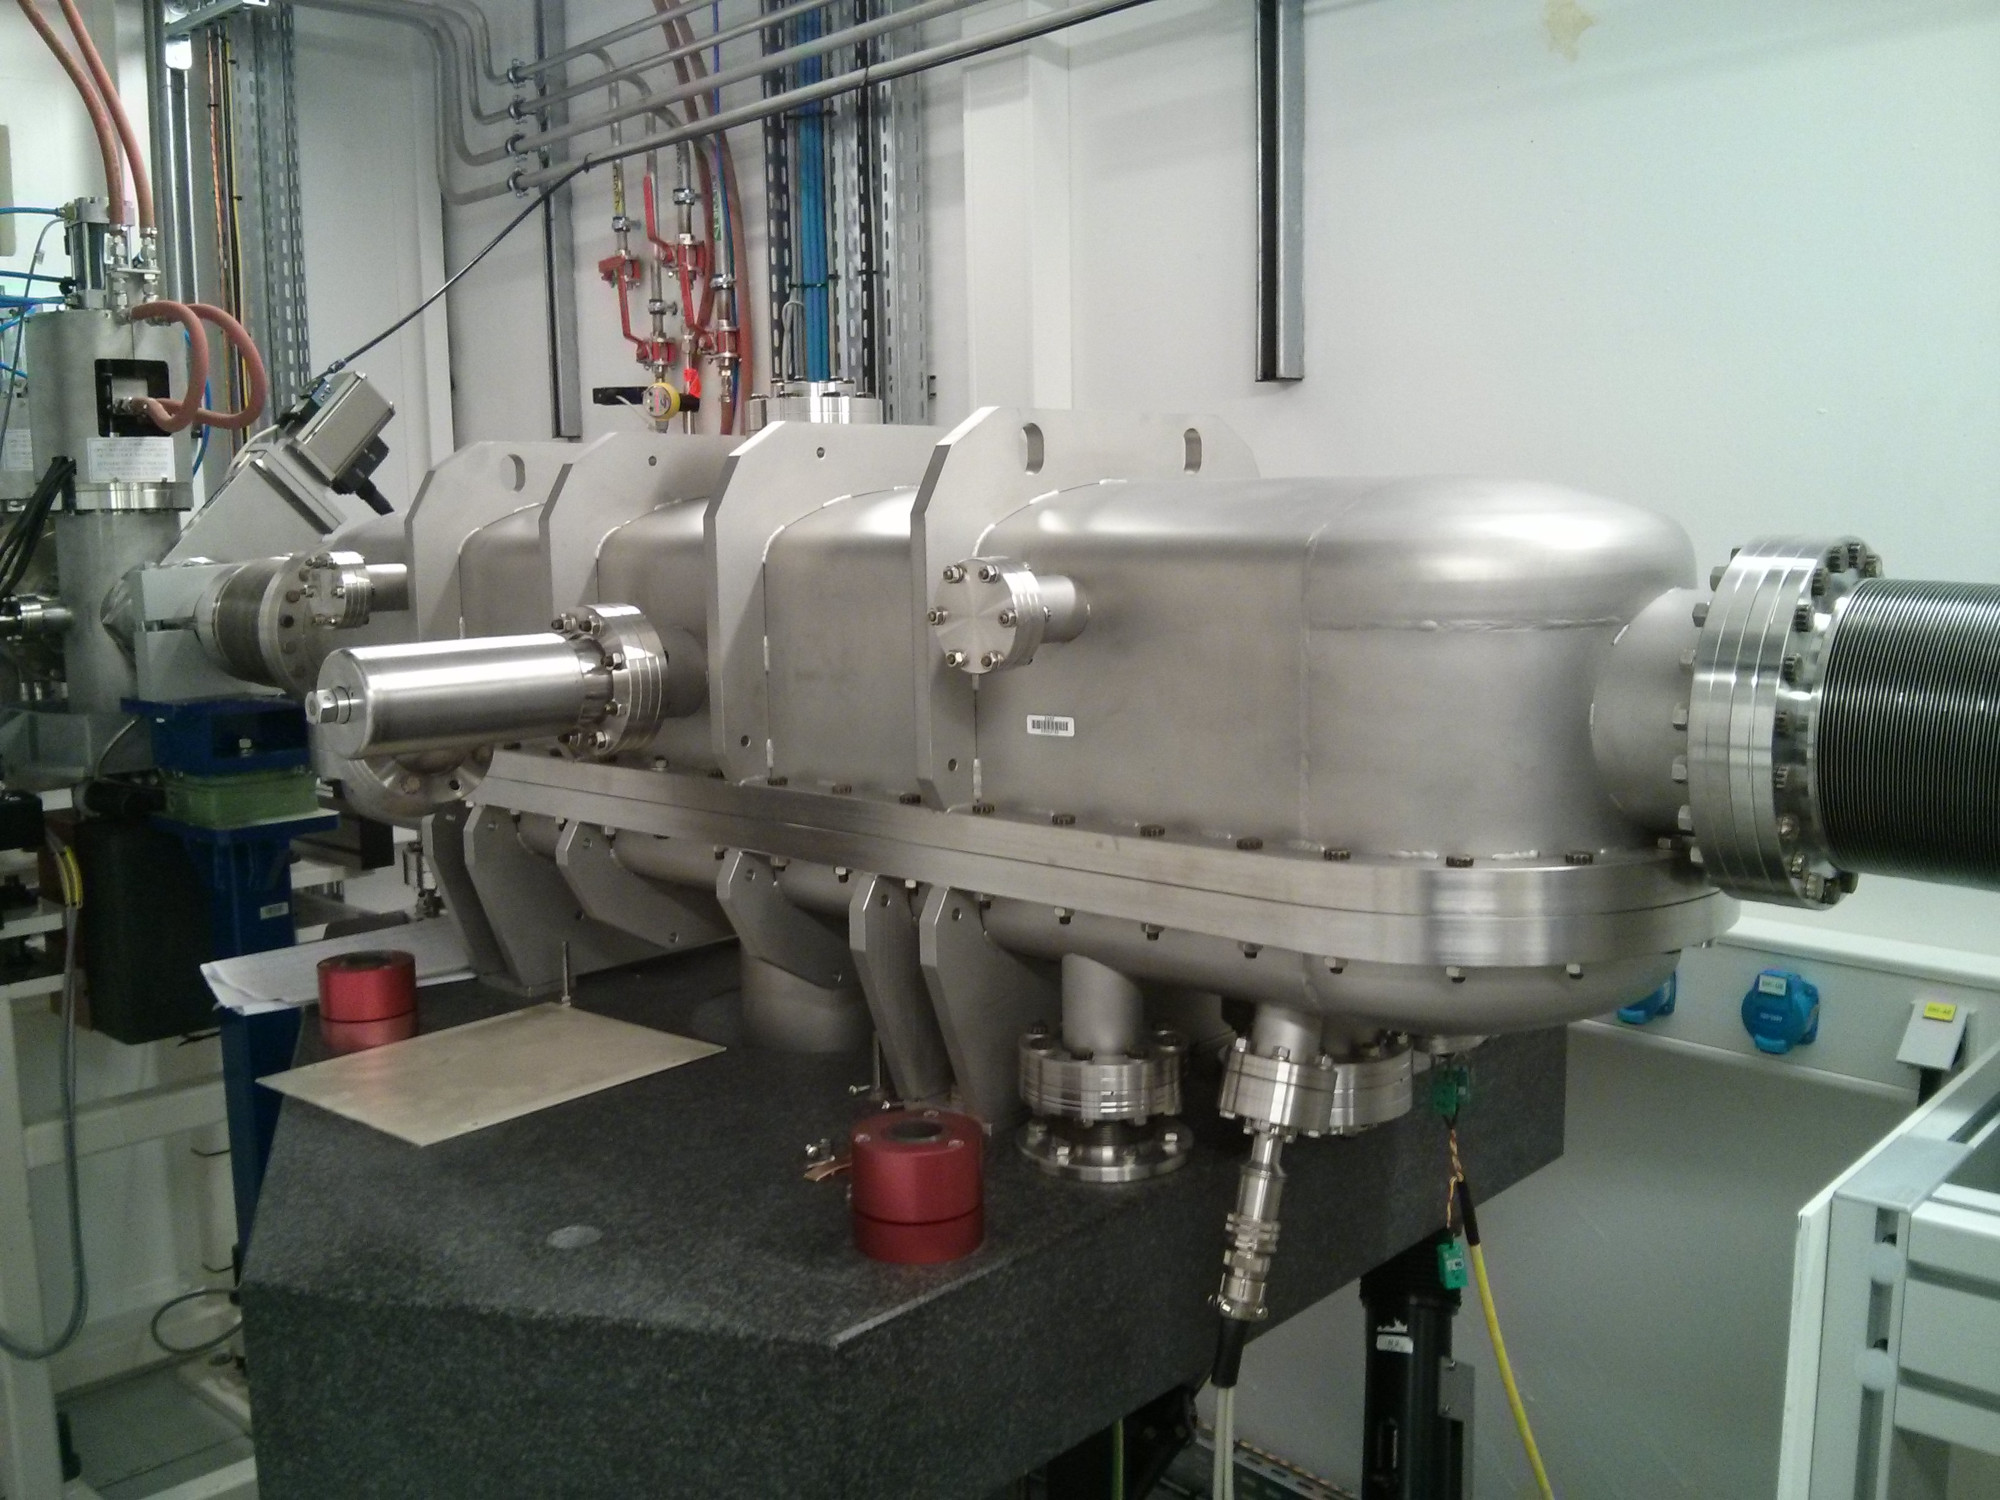
\includegraphics[scale=0.11]{Images/IMG_20151210_202740.jpg}
        \caption{Diffraction grating}
        \label{Reseau_diffract}
    \end{center}
\end{figure}


Now, the X-Ray coming from the storage ring have been modified to fit to the exact parameters we want, it thus goes through another room, where all measurement facilities are available. The measure is quite simple, we just need to put our sample in the beamline (figure \ref{ligne_mesure}) and measure X-Ray intensity before the sample and after the sample. The intensity difference gives us the X-Ray absorded while crossing our sample.

\begin{figure}[H]
    \begin{center}
        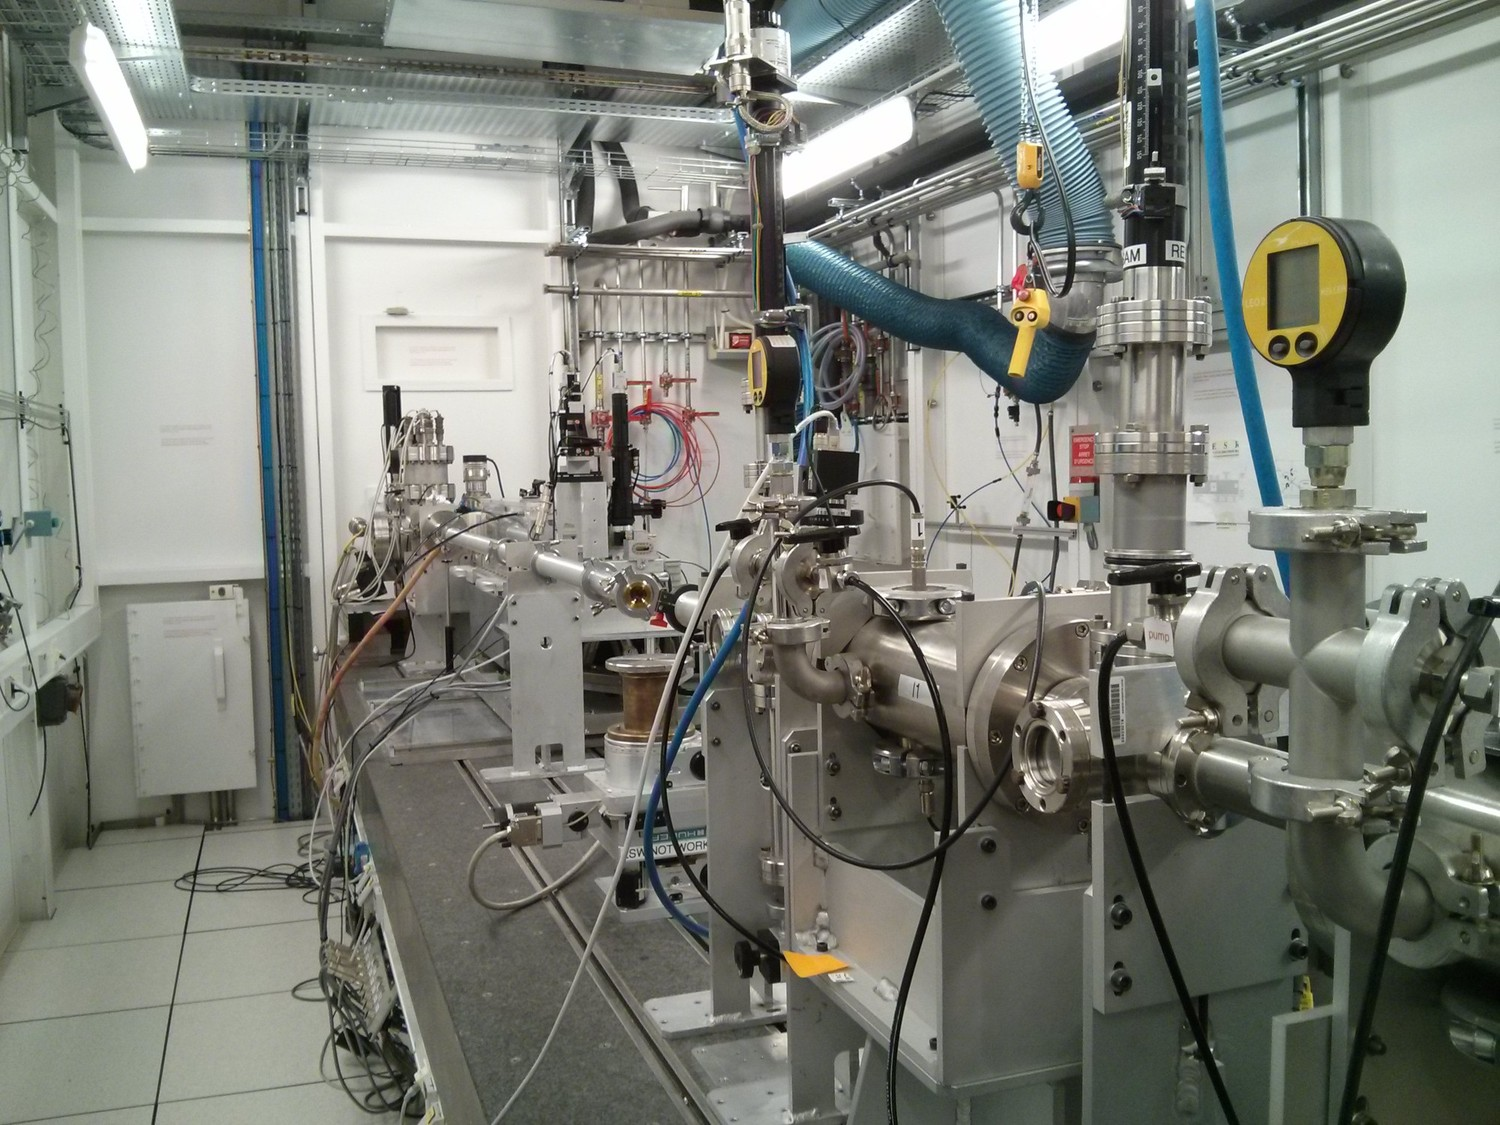
\includegraphics[scale=0.07]{Images/IMG_20151210_203229.jpg}
        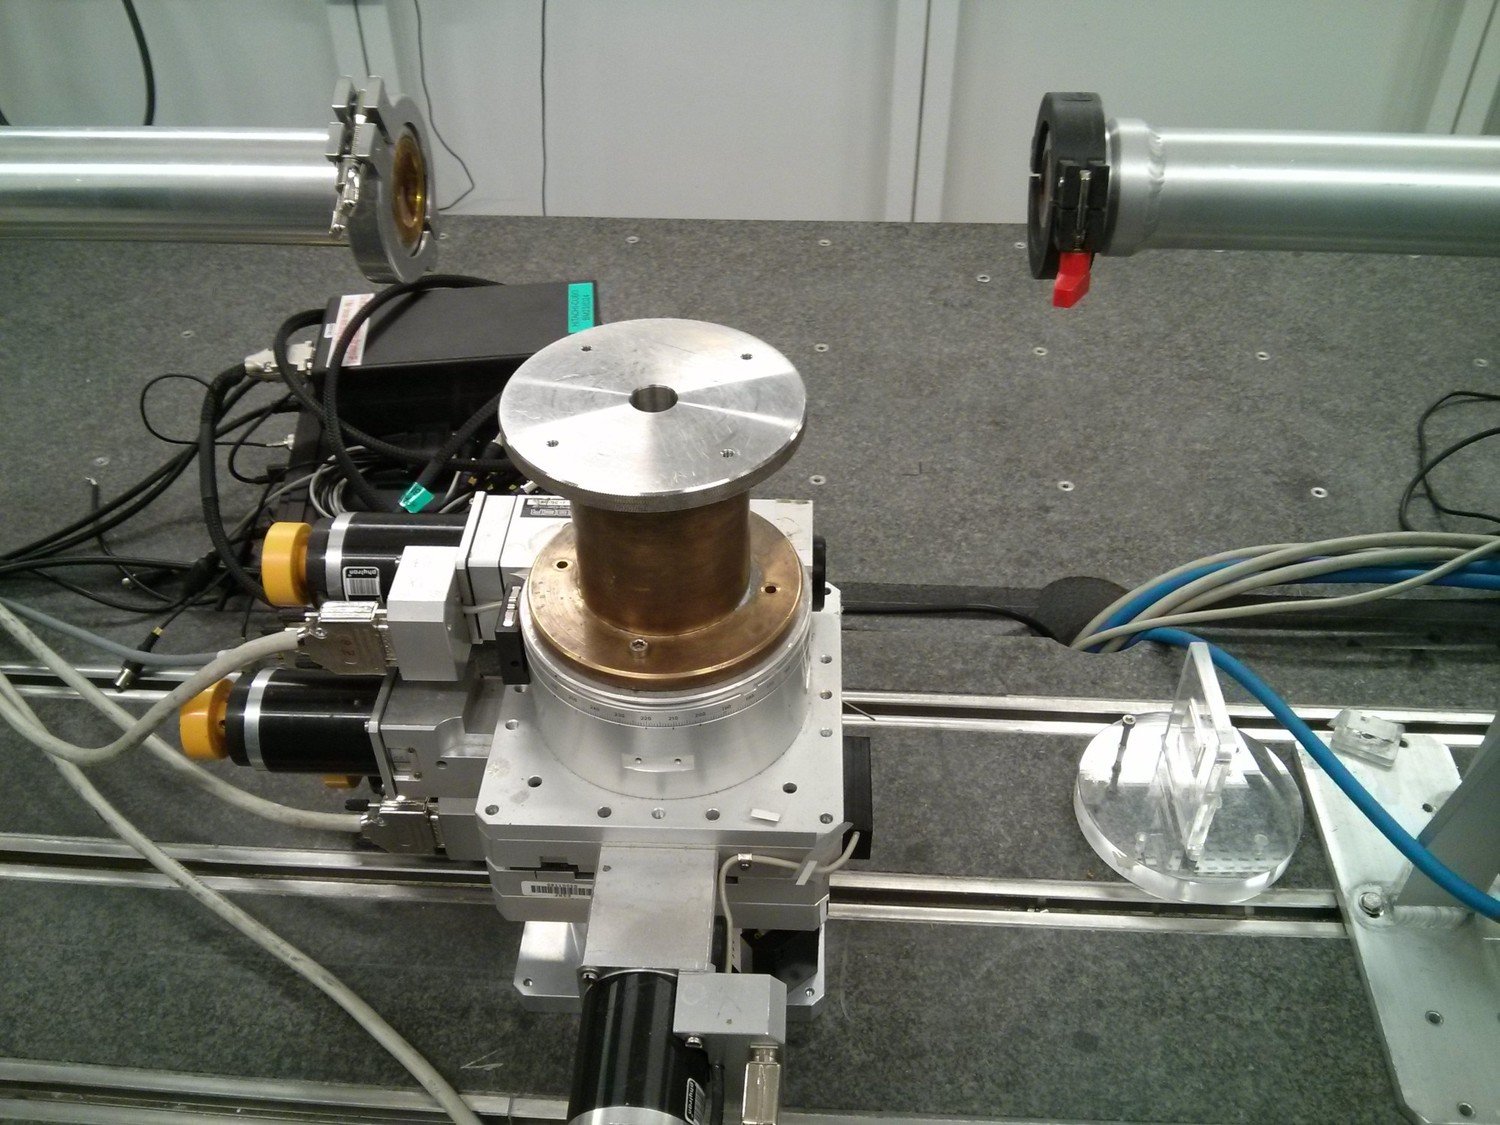
\includegraphics[scale=0.07]{Images/IMG_20151210_203316.jpg}
        \caption{Experimental cab}
        \label{ligne_mesure}
    \end{center}
\end{figure}


\section{Safety}\label{Safety}
As we have seen earlier, X-Ray can interact with matter and atoms, and because at ESRF they are quite energetic, X-Rays are dangerous. This is why there are some safety measures that were put in place to guarantee the safety of ESRF employees and researchers. In addition of standard measures such as emergency procedure, evacuation there is a part in safety rules concerning radiation protection, and how the site is made to avoid employees to be exposed to radiations, and a large part concerning the beamlines, where the risks are high.

There is a control panel (Figure. \ref{SafetyPanel}) at each beamline entrance, which informs if the shutter is closed or not, if the entrance is allowed or not so that everyone can know if it is safe to enter. The hutch is closed if the shutter is open and the door of the hutch can be opened only if the shutter is closed, so that noone can enter if the shutter is open.

\begin{figure}[H]
\centering
    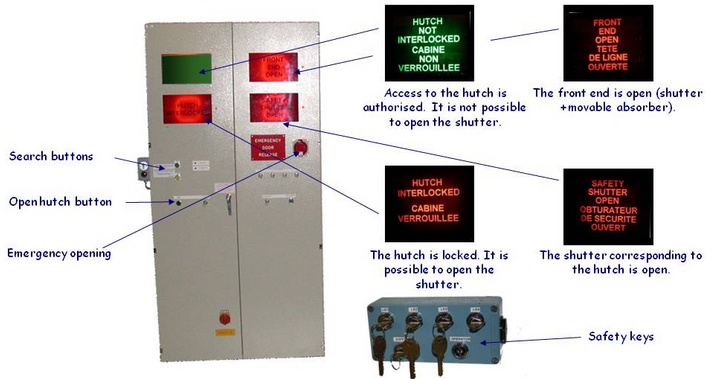
\includegraphics[width=350pt]{Images/SafetyPanel.png}
    \caption{Safety Panel\cite{Safety}}
    \label{SafetyPanel}    
\end{figure}

Whenever anyone exits a hutch, a search must be performed, in order to check if anyone stayed inside the hutch. There is a button to start a search, and a button inside the hutch to press, to be sure the search has been realized. Then, it is possible to end the search and close the hutch door. Inside the hutch, there also are emergency buttons to rapidly close the shutter to prevent any problem.


\section{EXAFS Domain and utilization}
In this part, we will explain the principles of EXAFS measurements.

\subsection{Atomic X-Ray absorption}

When interacting with matter, X-Rays are absorbed by atoms, resulting into an electron excitation.

If the incident X-Ray beam has a greater energy than the binding energy of a core-level electron, this electron is ejected from the atom into the continuum, leaving the atom with a core hole\cite{Pres}.\\This is the Photoelectric effect.

The atom will relax from this excited state through two main processes : X-Ray Fluorescence and Auger Effect.

\paragraph{The Auger Effect :} To fill the core hole, an electron drops into it. The dissipated energy is asborbed by a second electron, thus ejected from a higher energy core-level into the continuum.

\paragraph{The X-Ray Fluorescence :} As in the Auger Effect, an electron drops into the core hole from a higher energy core-level, while emitting an X-Ray beam of the energy gap between the core levels.

Those two effects result into a quasi-linear absorption coefficient :
\[\mu \simeq \frac{\rho Z^4}{A E^3}\]
\begin{figure}[H]
    \begin{center}
        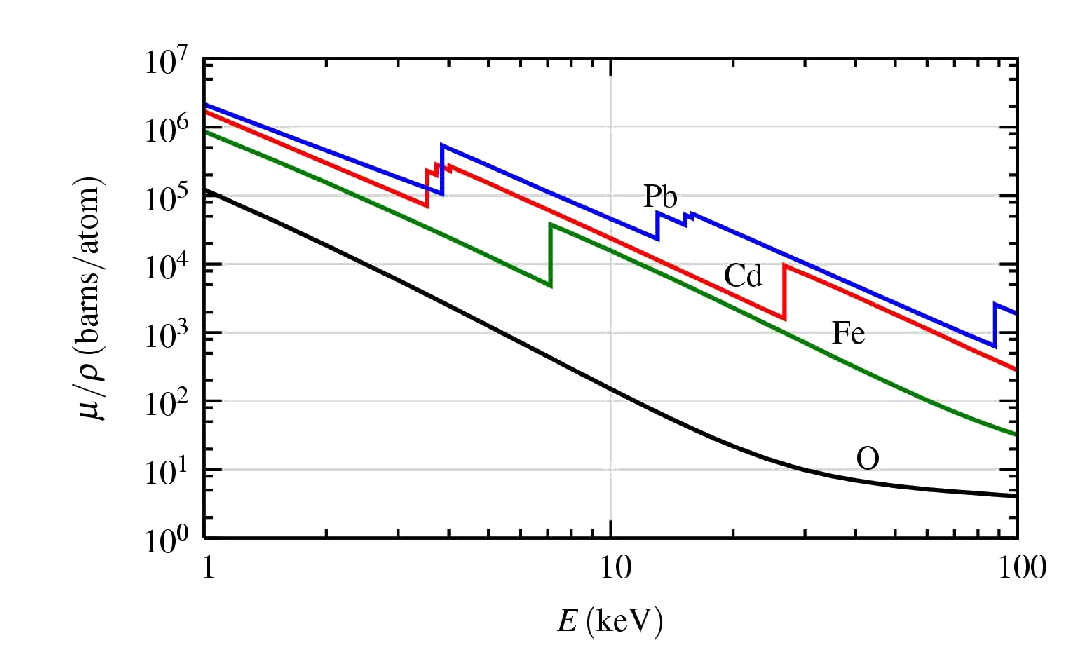
\includegraphics[width=0.7\textwidth]{Images/AbsorptionCoeff}
        \caption{The X-Ray absorption coefficient for Pb, Cd, Fe and O.}
        \label{absorptionCoeff}
    \end{center}
\end{figure}

The "edges" in this graph result from the electronic energy levels of the element : for each edge, another core level can absorb the X-Ray, as the incident energy became enough to excitate the level.

\subsection{The XAFS phenomenon}
For an isolated atom, the absorption edges are perfectly sharp, and $\mu(E)$ is smooth above the edges.

But in condensed matter, the absorbing atom is surrounded by other atoms (same or different) : the emitted photo-electron can scatter from neighboring atoms and come back to the first atom.

The outgoing and ingoing waves of the back-scattered photo-electron will interfere, thus modulating the absorption coefficient of the atom (Fig. \ref{scatteringschema}).
\begin{figure}[H]
    \begin{center}
        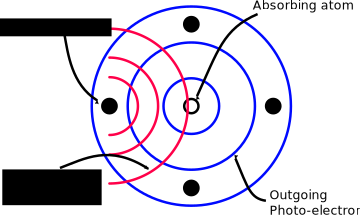
\includegraphics[width=0.5\textwidth]{Images/Scattering}
        \caption{A photo-electron emitted (blue) and back-scattered (red) to the central atom}
        \label{scatteringschema}
    \end{center}
\end{figure}

This modulation is easily visible on the Figure \ref{exafsgraph}. We will define the normalized EXAFS oscillations :
\[\chi(E) = \frac{\mu(E) - \mu_0(E)}{\Delta\mu_0(E_0)}\]
with $\mu_0(E)$ the "smooth background" of the isolated atom, and $\Delta\mu_0(E_0)$ the edge step or "jump".

\begin{figure}[H]
    \begin{center}
        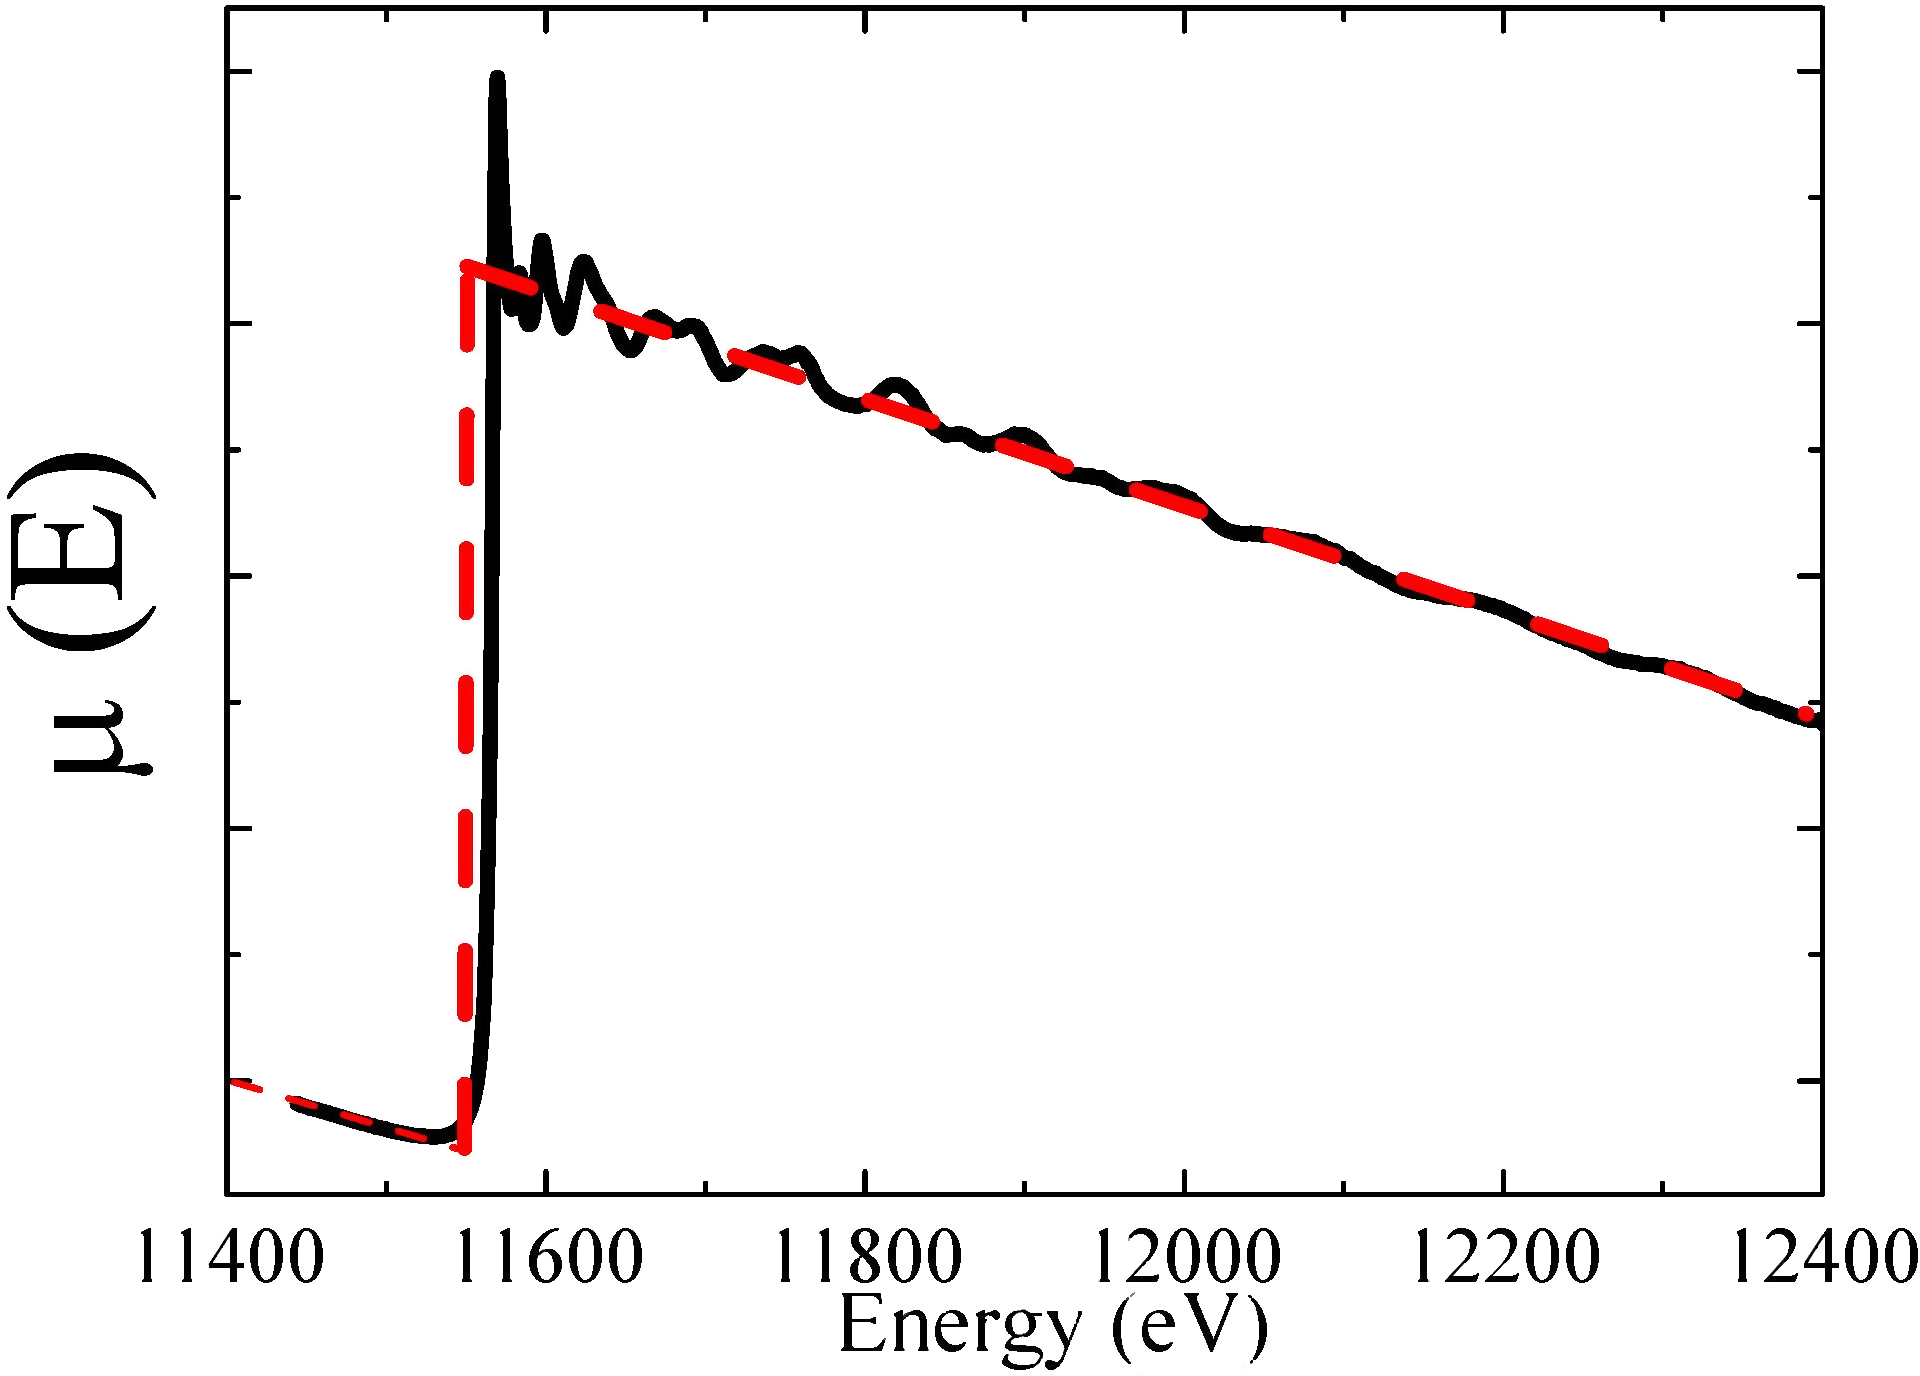
\includegraphics[height=0.35\textwidth]{Images/EXAFS2}
        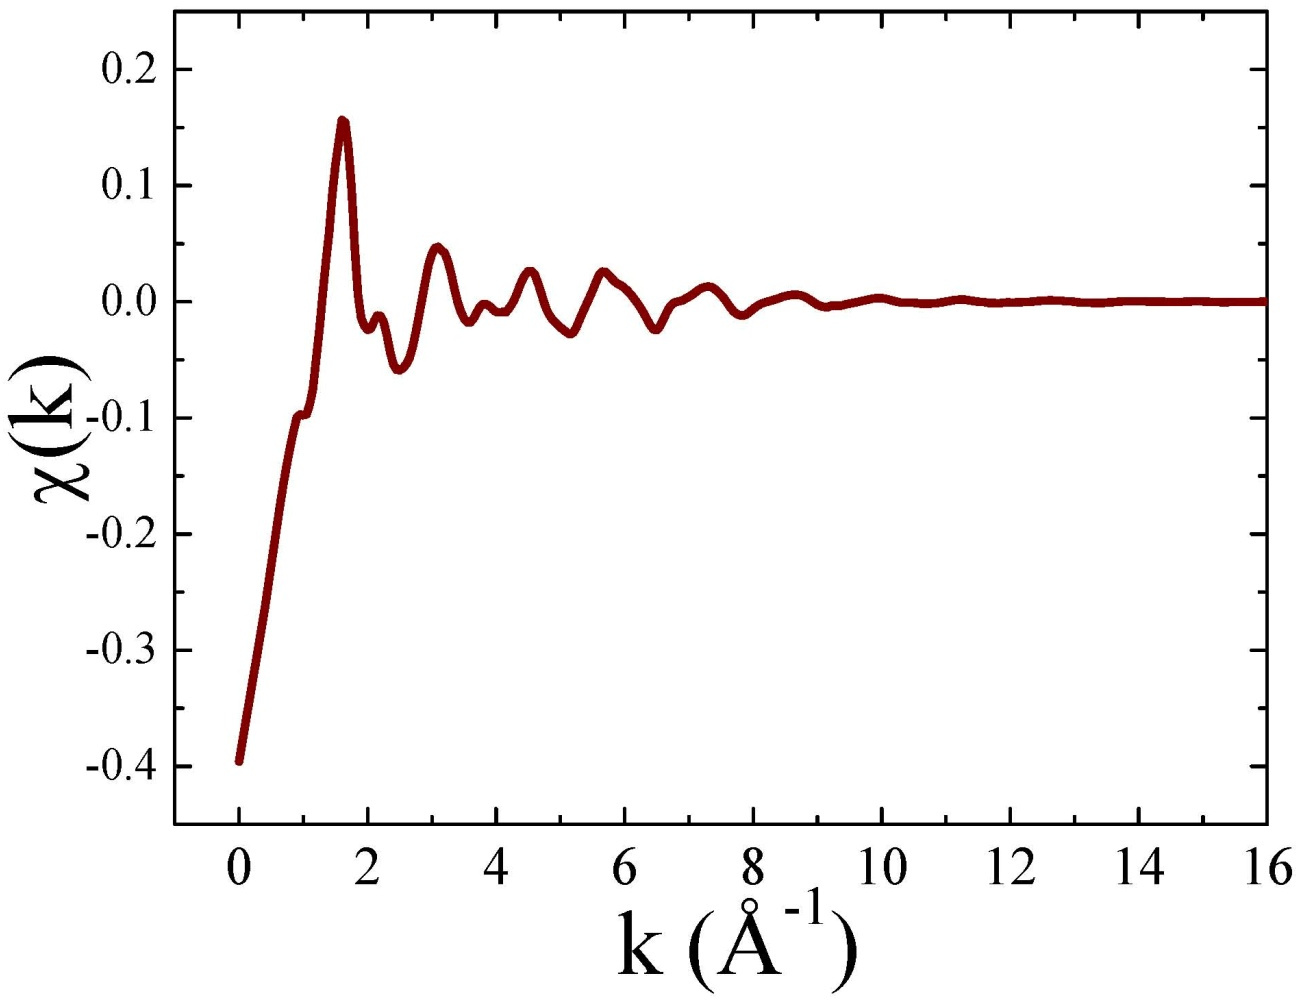
\includegraphics[height=0.35\textwidth]{Images/relativeEXAFS}
        \caption{EXAFS phenomenon, raw and normalized}
        \label{exafsgraph}
    \end{center}
\end{figure}

\chapter{Experimental measurements}

\section{Experimental protocol}
In this part, we will briefly show how to initiate an experiment, by the fabrication of an sample and the preparation of the beamline to begin the measurements.

\subsection{Cu$_2$O sample construction}

For the measurements, we need several samples to be able to make comparison between them. The first sample was made of Copper and was already ready. We also realized a pellet of Cu$_2$O, that we made.

 We mixed a precise weight of two powders, to dilute Cu$_2$O, since a small amount is enough (as told by a software on the computer) with a mortar and pestle (Fig. \ref{MixMortier}) to make an homogeneous light pink powder.

\begin{figure}[H]
    \centering
    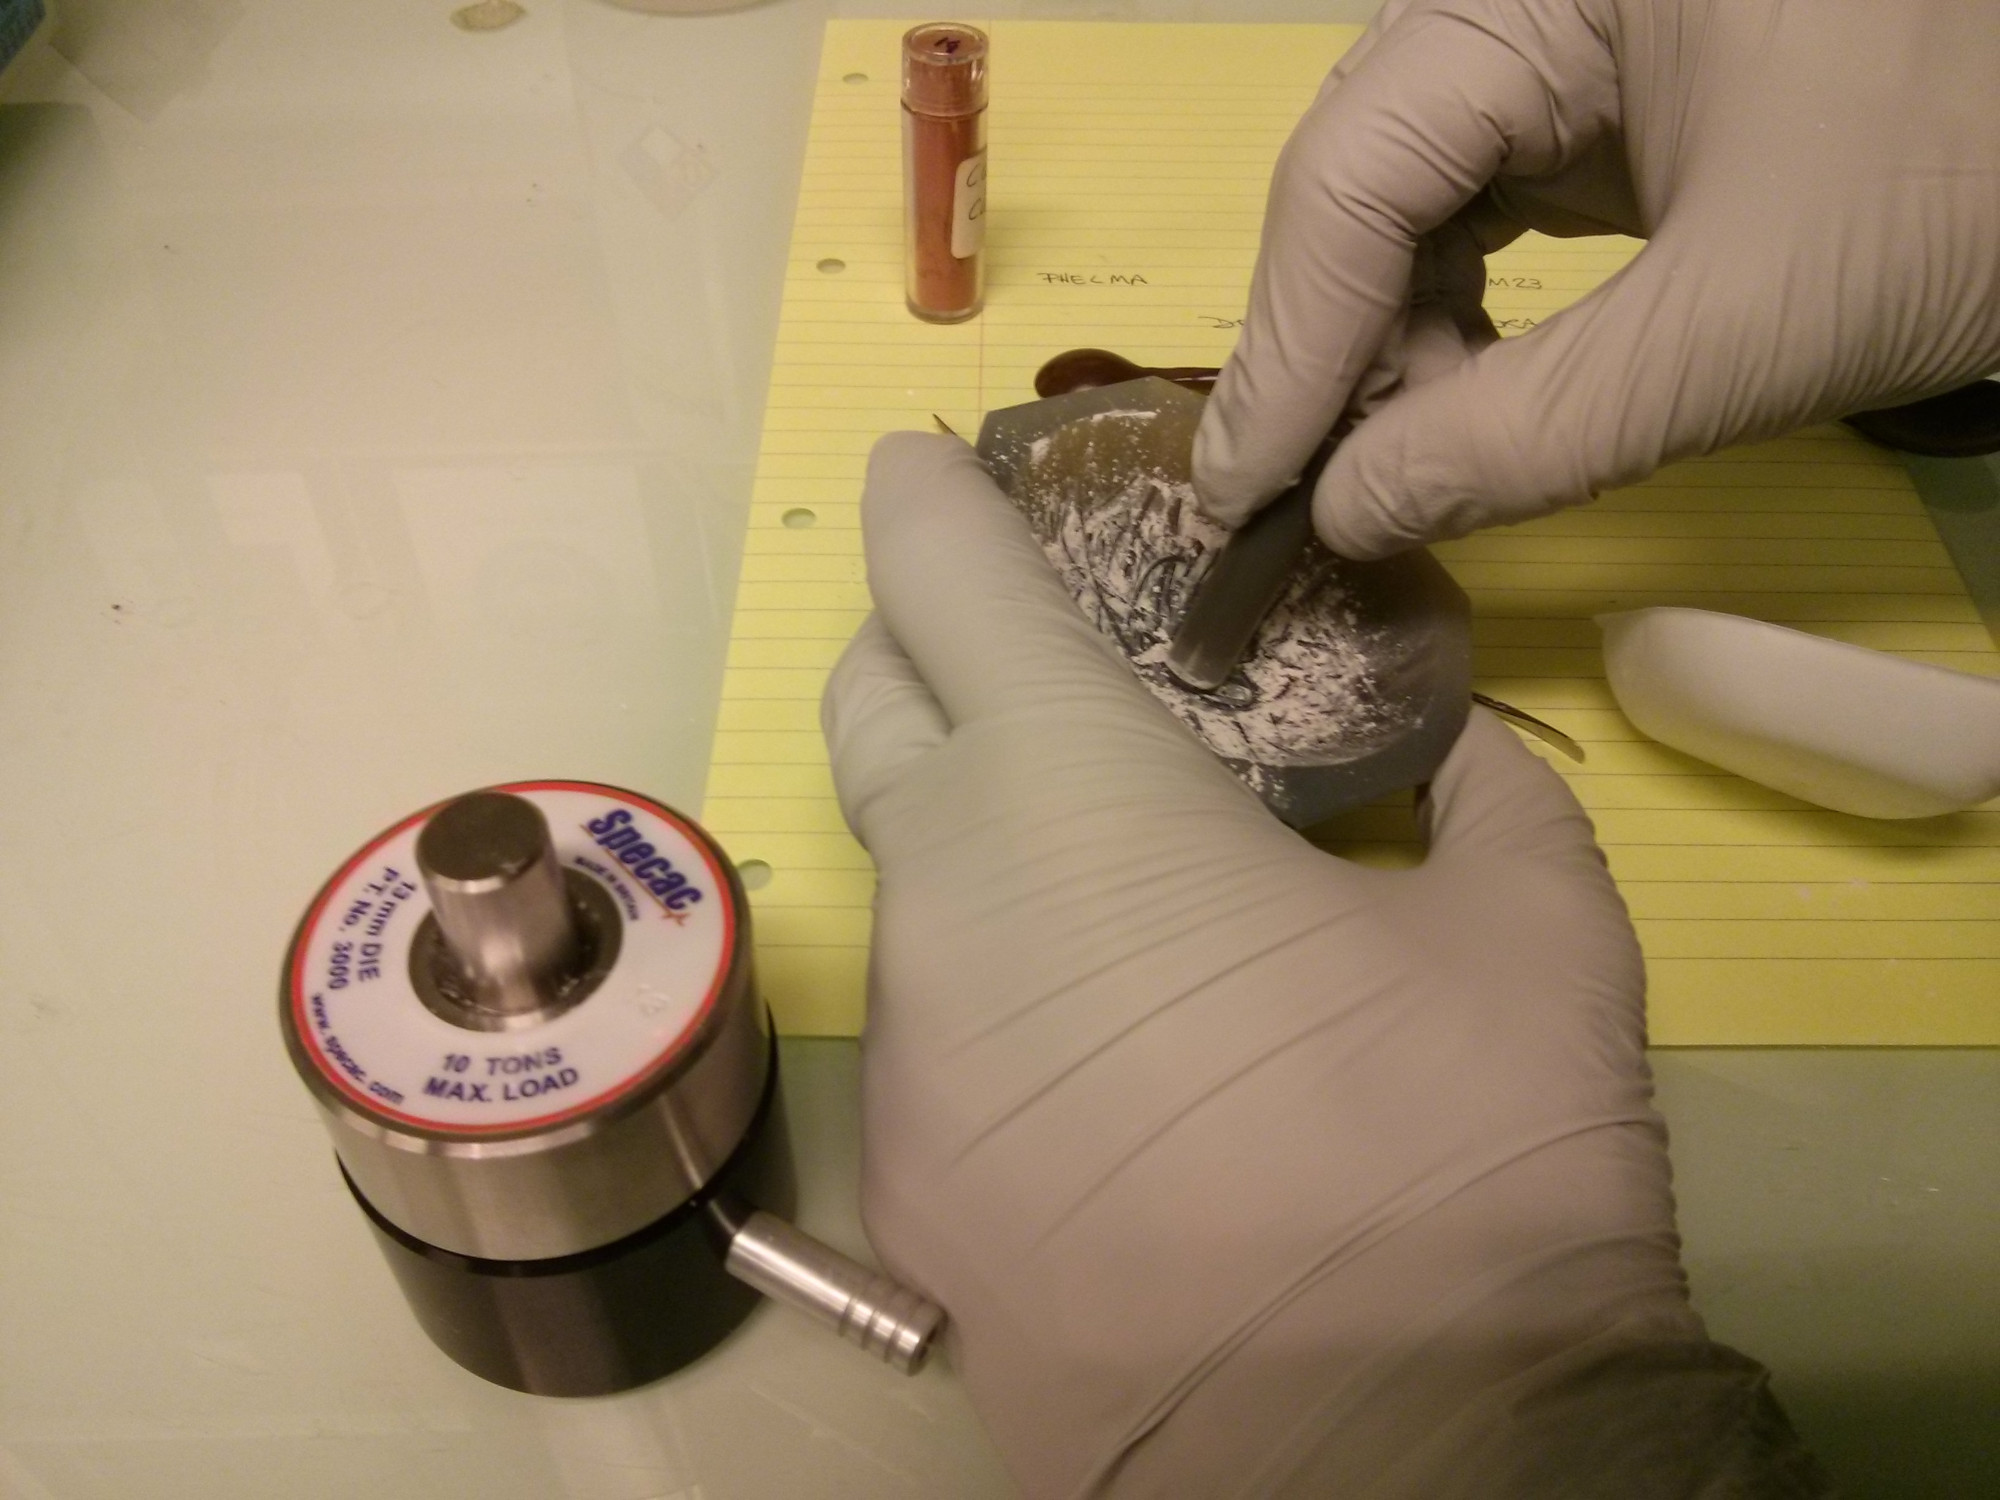
\includegraphics[width=250pt]{Images/pellet1.jpg}
    \caption{Making an homogeneous powder}
    \label{MixMortier}
\end{figure}


Then, we put this powder in a press, to create a pellet by submitting the powder to a high pressure. Finally, we put the pellet in a sample holder, carefully to avoid to break it (Figure \ref{pellet}).

\begin{figure}[H]
\centering
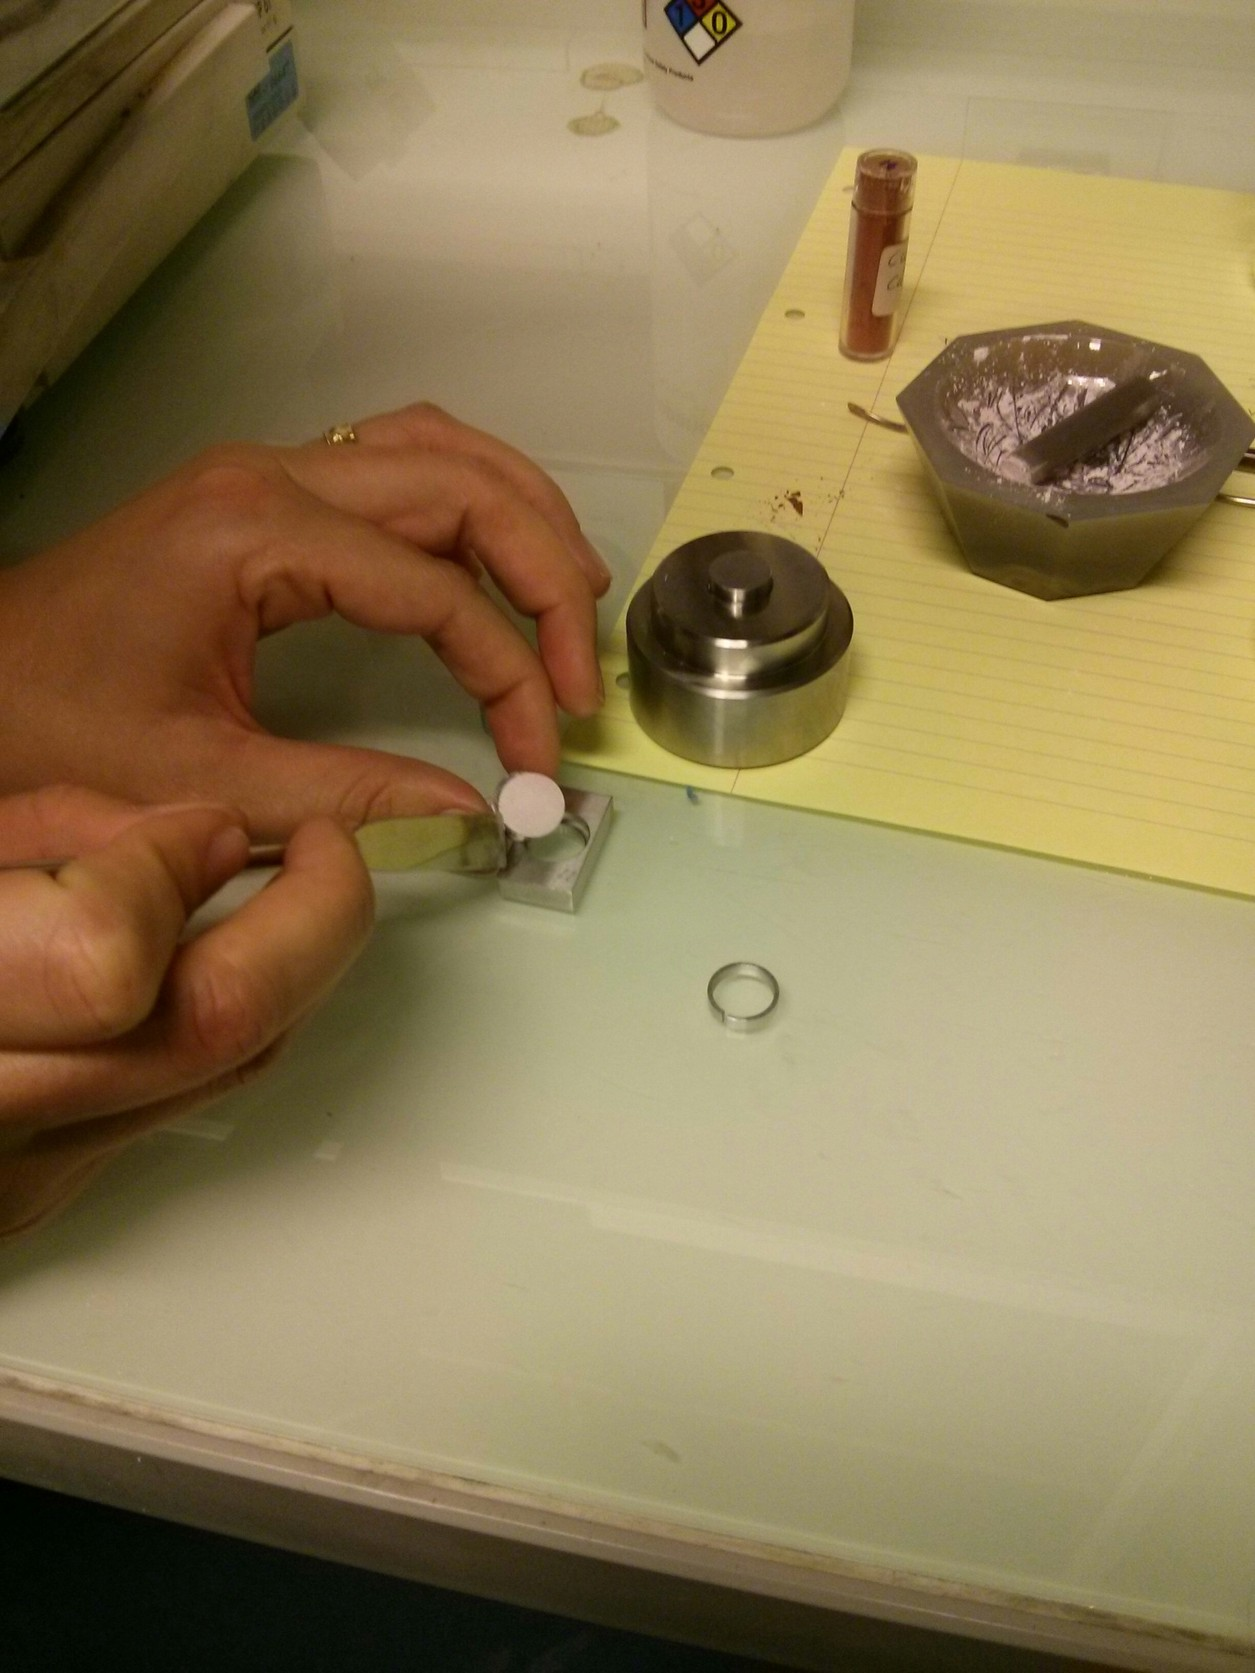
\includegraphics[width=200pt]{Images/pellet2.jpg}
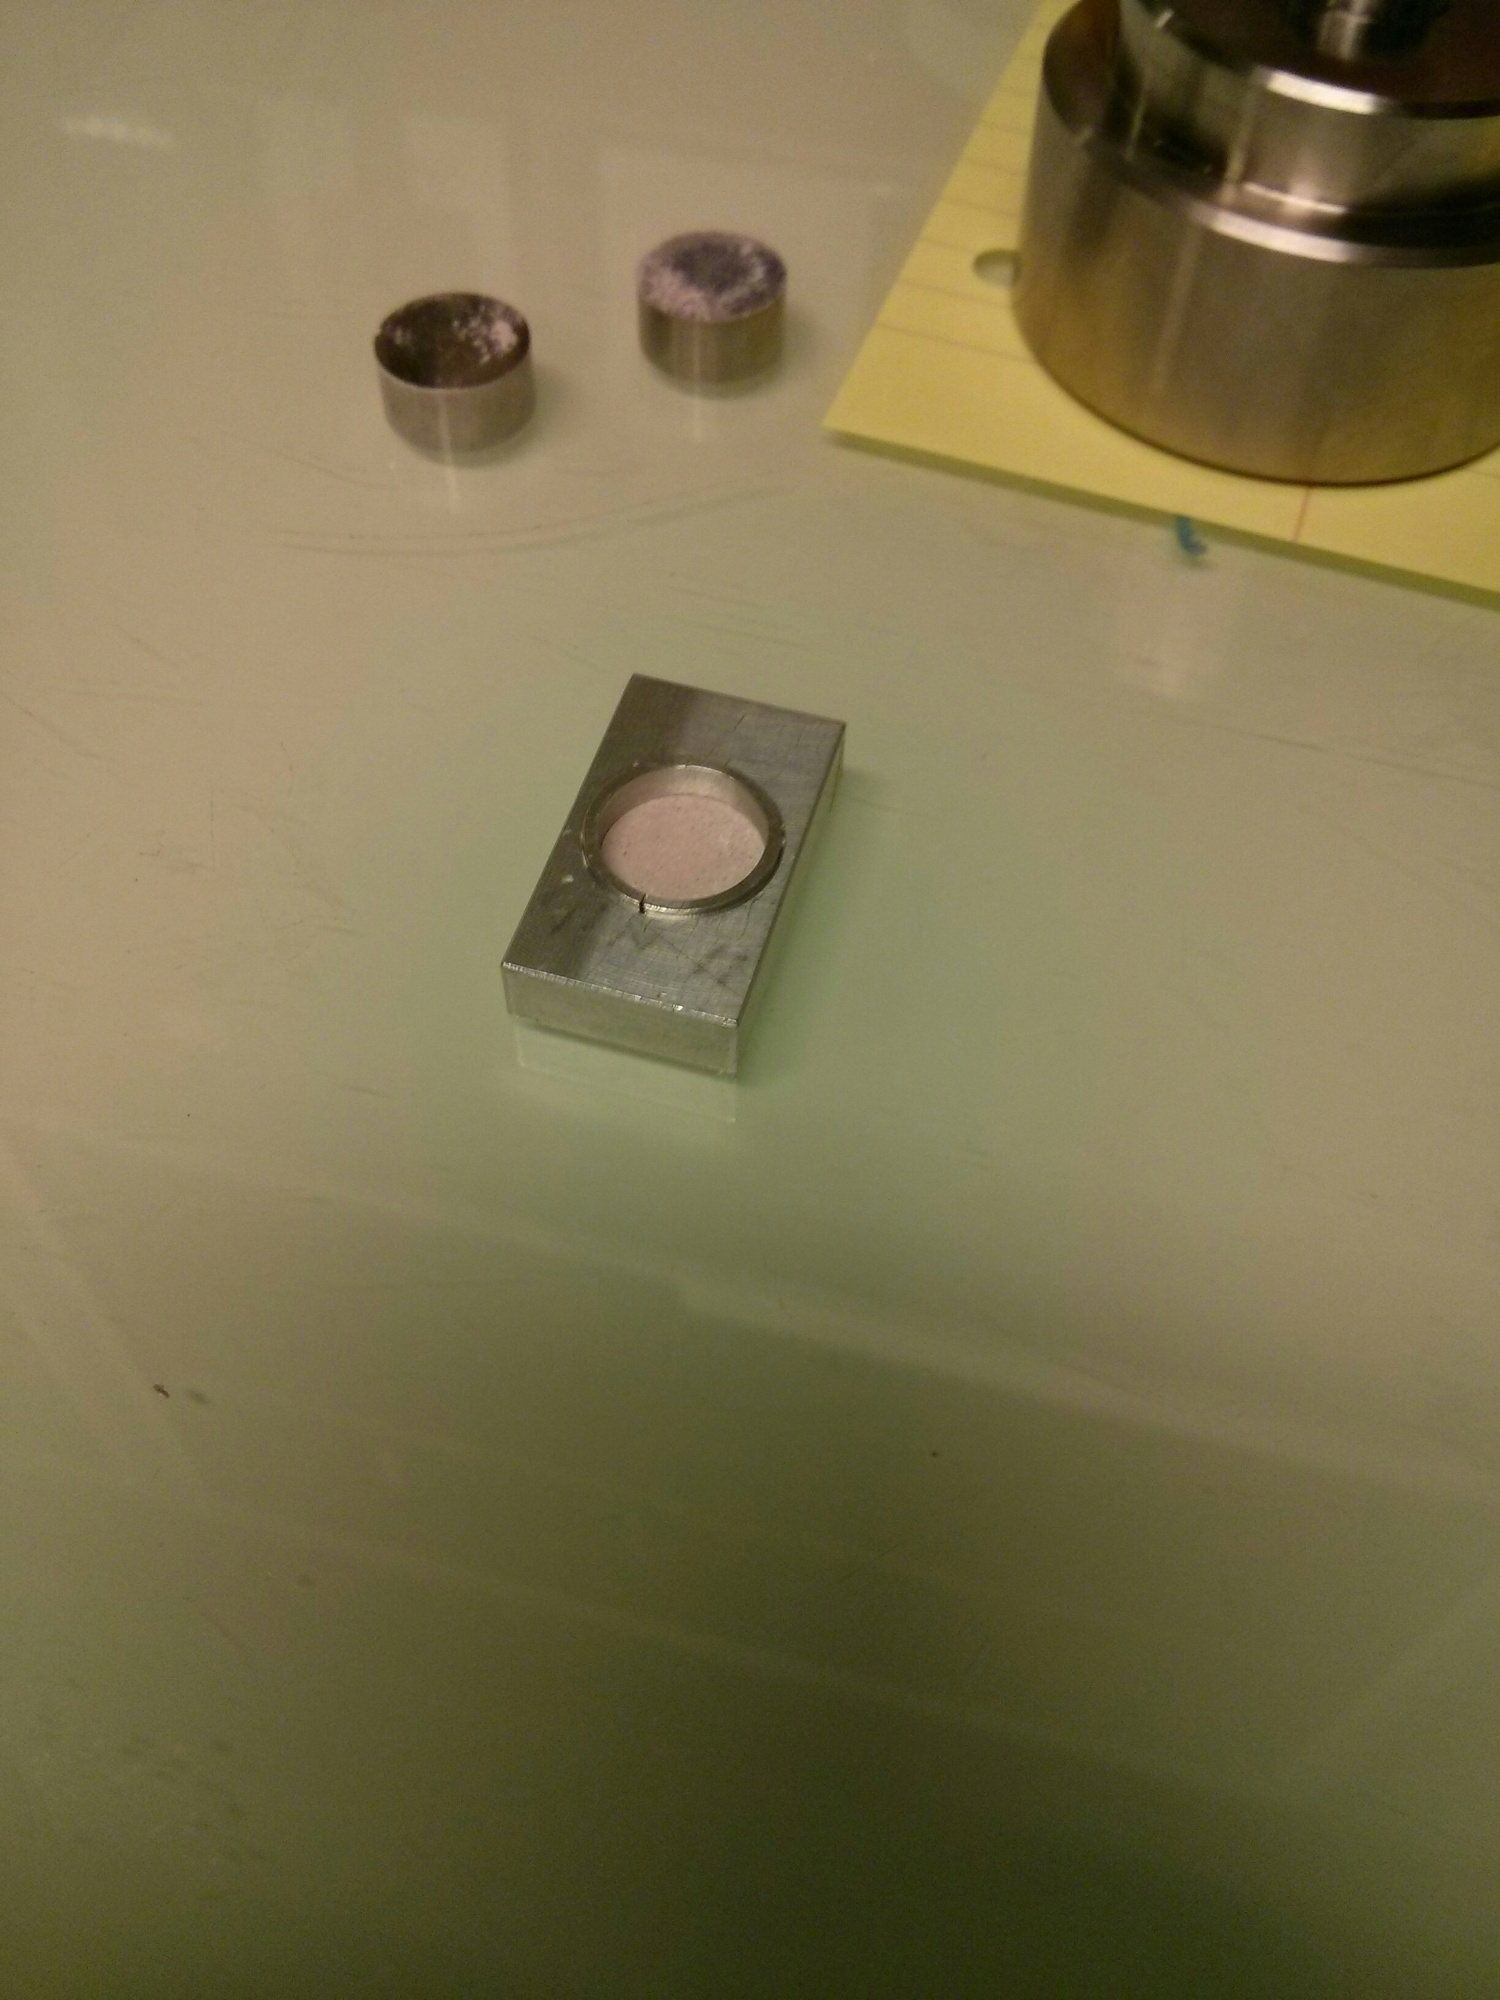
\includegraphics[width=200pt]{Images/pellet3.jpg}
\caption{Finalization of the creation of the pellet}
\label{pellet}    
\end{figure} 

For the measurements, we used a Copper pellet, a Cu$_2$O pellet and a CuO pellet (made by the previous group).

\subsection{Preparation of the beamline}

First of all, before starting any measurements on samples, we need to place the sample in the beamline where X-Rays will be able to cross it and interact with the atoms. For this when need to enter in the hutch, respecting the Safety Measures (See \ref{Safety}). We place the sample at the place made for this. We pump to remove air, and replace it with other gases (A mix between Nitrogen and Helium) thanks to different gases lines available. Then we can go out of the hutch, open the shutter and start the measurements.

\section{Results of measurements and graph analysis} \label{results}

The different samples presented earlier and another sample of Cu$_2$O prepared by the first group have all been analysed using the EXAFS technique. The results are presented and discussed below. All these graphs shows the absorption of copper atoms, since oxygen does not absorb X-Ray very well.

\subsection{Absorption graph}
The figure \ref{graph1} presents the absorption graph of the three samples. The normalized absorption is plotted versus the X-Ray beam energy. Despite they have a similar composition with the same atoms involved, the three samples have a different absorption at the same energy. The influence of neighbouring atoms can be seen in this first plot, and the interaction of the photo-electron generated are quite different depending on the structure of the material.
\begin{figure}[H]
    \begin{center}
        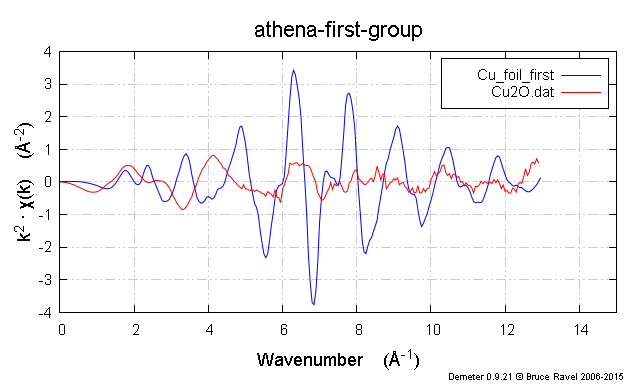
\includegraphics[width=0.7\textwidth]{ImagesTP/image2}
        \caption{Absorption graph of the three samples}
        \label{graph1}
    \end{center}
\end{figure}

Figure \ref{graph2} shows absorption function plotted versus wavenumber k. The dependence between the energy and the wavenumber of the X-Ray is given by   with Wk the ionization energy of the atom.
Absorption also depends strongly on the material analysed. The pure Cu foil (red curve) shows oscillations with a much higher amplitude than the two oxides. The two oxides signals also present an important noise, especially CuO. The explanation can be a non-uniformity of the concentration of CuO in the sample.
\begin{figure}[H]
    \begin{center}
        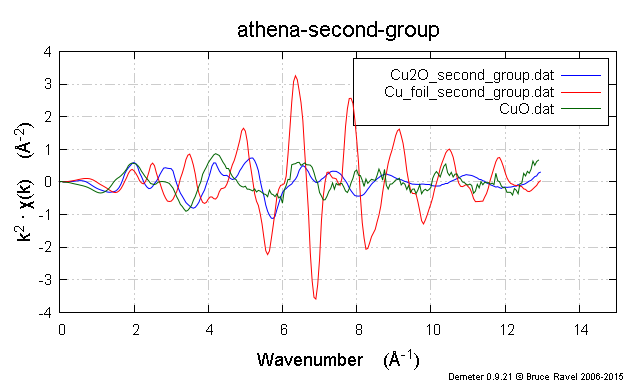
\includegraphics[width=0.7\textwidth]{ImagesTP/image4}
        \caption{Absorption function versus wavenumber}
        \label{graph2}
    \end{center}
\end{figure}

\subsection{Neighbours distance graph}
Now the previous curves can be used to check which neighbours does copper atoms see in the structure of the material. A Fourier transform is performed on the absorption function curves (Fig.\ref{graph2}). So the absorption can now be plotted versus a radial distance as shown in figure \ref{graph3}. The curves obtained have all several peak corresponding to the interaction between the photo-electron and the different neighbours of copper atoms in the structure. To find out which peak correspond to which interaction, these curves are crossed with a database which can be found online. Every interaction between copper and other atoms has his own signature previously measured and classified. That means that the interactions must be predicted depending on the analysed sample. These interactions are then checked one by one.



\begin{figure}[H]
    \begin{center}
        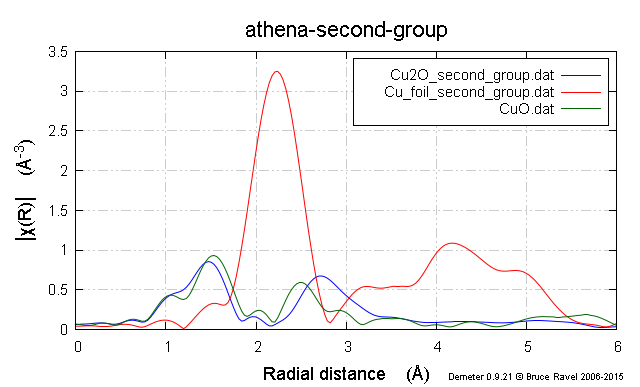
\includegraphics[width=0.7\textwidth]{ImagesTP/image6}
        \caption{Absorption versus radial distance}
        \label{graph3}
    \end{center}
\end{figure}


First of all, let’s have a closer look to the copper foil curve. Since the sample only contains copper, it seems obvious to consider the interaction between two copper atoms, where the photo-electron goes to another copper atom then comes back to the first copper atom. The figure \ref{graph4} shows in red this interaction compared to the Cu foil EXAFS curve. There is a match between the Cu foil higher peak and Cu 1.1 interaction curve. The peaks on the left of this main peak seems to be explainable with this interaction too. But the right part of the curve does not match really well. However, it can be explained by other interaction between three or more copper atoms, or with the second or more nearest copper atom. The photo-electron can for example go to a second copper atom, then to a third and back to the first. These interactions have been checked and confirmed, but are not plotted in this report.

\begin{figure}[H]
    \begin{center}
        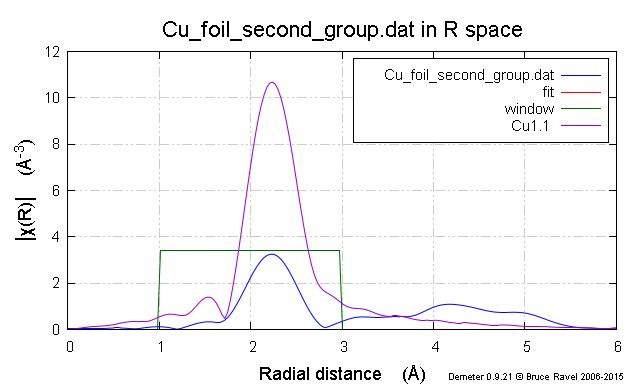
\includegraphics[width=0.7\textwidth]{ImagesTP/image7}
        \caption{Interaction between Copper atoms}
        \label{graph4}
    \end{center}
\end{figure}

The same analysis has been made with the Cu2O oxide sample, the results are plotted on figure \ref{graph5}. The same interaction between two coppers is checked, along with the interaction between a copper atom and an oxygen atom. As predicted, there is a match for both of them. The two main peaks of the oxide curve, along with the one between them, correspond to the green or purple curve. With the same idea than with the copper foil, the rest of the curve is explained by more complicated interactions, with an atom of copper and then an atom of oxygen for example.
\begin{figure}[H]
    \begin{center}
        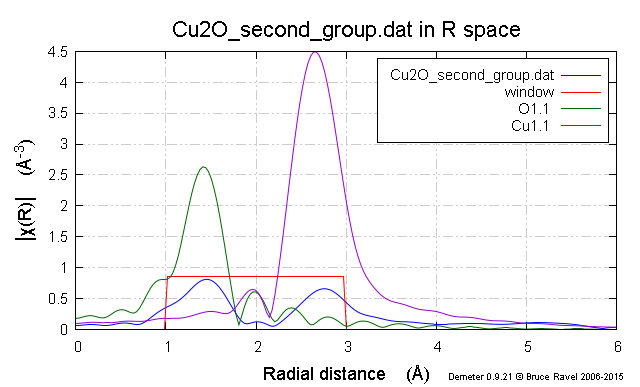
\includegraphics[width=0.7\textwidth]{ImagesTP/image8}
        \caption{Interaction between atoms in Cu$_2$O sample}
        \label{graph5}
    \end{center}
\end{figure}

\clearpage
\newpage

\chapter*{Conclusion}
\addcontentsline{toc}{chapter}{Conclusion}

	This practical work allowed us to learned a lot about how a synchrotron works and about how to make experiments in such a big structure. We have learned about safety measures that are mandatory in a big scientific place where risks can be high while manipulating. Moreover, is has been a great experience to make an experiment in an important and unique research place like ESRF.
		
	We were also able to make our own samples, characterize the matter within them and compare several different samples. The study of EXAFS results allowed us to compare the spectral absorption of our Cu$_2$O sample with these of a Cu sample reference and the data files made it possible to analyze the composition of our sample. 
	
	Even if the experiment was not revolutionnary (which was not the goal) it made us understand the basics of EXAFS measurements and the exploitation of the results obtained : how to interpret graphs and determine the structure of the matter and the atoms in the sample.

\nocite{*}
\bibliographystyle{unsrt}
\bibliography{Biblio}
\end{document}
